\documentclass[crop,tikz]{standalone}
\usepackage{amsmath}
%\usepackage[french]{babel}
\usepackage[utf8]{inputenc}
%\usepackage[T1]{fontenc}
\usetikzlibrary{positioning}
\usetikzlibrary{shapes,backgrounds}

\newcommand{\tstar}[5]{% inner radius, outer radius, tips, rot angle, options
\pgfmathsetmacro{\starangle}{360/#3}
\draw[#5] (#4:#1)
\foreach \x in {1,...,#3}
{ -- (#4+\x*\starangle-\starangle/2:#2) -- (#4+\x*\starangle:#1)
}
-- cycle;
}

\begin{document}
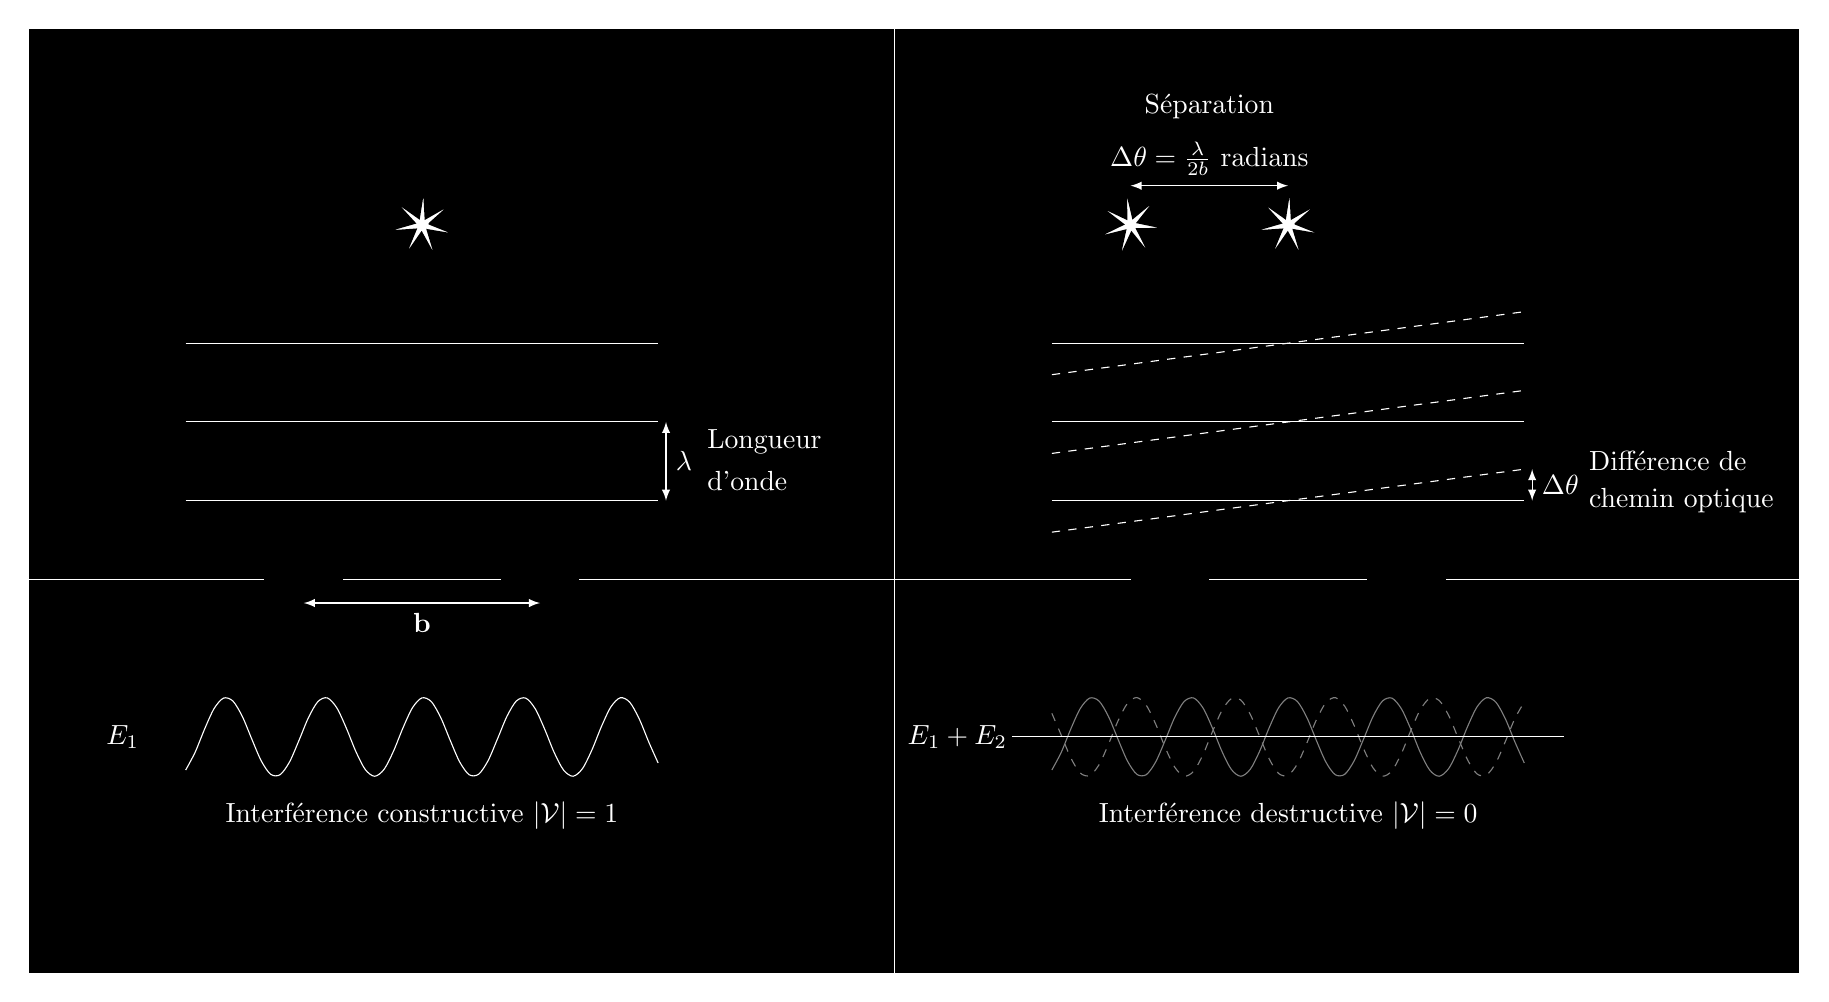
\begin{tikzpicture}[]
        \begin{scope}[shift={(-5.5, 0)}]
                \draw[fill=black, draw=white] (-5, -6) rectangle (6, 6);
                \node (s1) at (0, 4) {};
                \begin{scope}[shift={(0, 3.5)}]
                        \tstar{0.1}{0.5}{7}{10}{thick,fill=white}
                \end{scope}
                
                \foreach \y in {0,...,2}
                {
                        \draw[draw=white] (-3, \y) -- (3, \y);
                }

                \draw[white] (-5, -1) -- (-2, -1);
                \draw[white] (6, -1) -- (2, -1);
                \draw[white] (-1, -1) -- (1, -1);


                \draw[latex-latex, white] (-1.5, -1.3) -- node[midway, below] {$\mathbf{b}$} (1.5, -1.3);
                \node[white] at (-3.8, -3) {$E_1$};
                \draw[color=white] plot[domain=-3:3,variable=\x,samples=51,smooth] ({\x},{0.5*sin(5*deg(\x+2.8)) - 3});
                \draw[white,latex-latex] (3.1, 1) -- node[midway, right] {$\lambda$} (3.1, 0);
                \node[white, anchor=west] at (3.5, 0.75) {Longueur};
                \node[white, anchor=west] at (3.5, 0.25) {d'onde};
                %\node[white] at (-4.2, -3) {$E_1$};
                \node[white] at (0, -4) {Interférence constructive $|\mathcal{V}| = 1$};
        \end{scope}
        \begin{scope}[shift={(5.5, 0)}]
                \draw[fill=black, draw=white] (-5, -6) rectangle (6.5, 6);
                \begin{scope}[shift={(0, 3.5)}]
                        \tstar{0.1}{0.5}{7}{10}{thick,fill=white}
                \end{scope}
                \begin{scope}[shift={(-2, 3.5)}]
                        \tstar{0.1}{0.5}{7}{20}{thick,fill=white}
                \end{scope}
                \node[color=white] at (-1, 5) {Séparation};
                \draw[latex-latex, color=white] (0, 4) -- node[midway, above, color=white] {$\Delta \theta = \frac{\lambda}{2b}$ radians} (-2, 4);
                \foreach \y in {0,...,2}
                {
                        \draw[draw=white] (-3, \y) -- (3, \y);
                        \draw[draw=white, dashed] (-3, \y - 0.4) -- (3, \y + 0.4);
                }
                \draw[white] (-5, -1) -- (-2, -1);
                \draw[white] (6.5, -1) -- (2, -1);
                \draw[white] (-1, -1) -- (1, -1);
                \draw[color=black!50,] plot[domain=-3:3,variable=\x,samples=51,smooth] ({\x},{0.5*sin(5*deg(\x+2.8)) - 3});
                \draw[color=black!50, dashed] plot[domain=-3:3,variable=\x,samples=51,smooth] ({\x},{0.5*sin(5*deg(\x+3.5)) - 3});
                
                \draw[white,latex-latex] (3.1, 0.4) -- node[midway, right] {$\Delta \theta$} (3.1, 0);
                \node[white, anchor=west] at (3.7, 0.5) {Différence de};
                \node[white, anchor=west] at (3.7, 0.) {chemin optique};
                
                \node[white] at (0, -4) {Interférence destructive $|\mathcal{V}| = 0$};
                \node[white] at (-4.2, -3) {$E_1 + E_2$};
                \draw[white] (-3.5, -3) -- (3.5, -3);
                %\draw[color=white] 
        \end{scope}
\end{tikzpicture}
\end{document}
